
\section{Capacitance Series Circuit}
%test comment
Name \rule{2.0in}{0.1pt}\hfill{}Section \rule{1.0in}{0.1pt}\hfill{}Date
\rule{1.0in}{0.1pt}

\textbf{Objective}

\begin{itemize}
\item To investigate the relationship among charge, potential difference, and capacitance in a series combination of capacitors.
\end{itemize}
\textbf{Introduction} 

In class the series combination of capacitors was studied with the assumption
of a constant potential difference energizing the circuit.  In practice this
is difficult to reproduce in the lab because capacitors typically do not
maintain a steady charge for very long.  To get around this we will energize
the circuit with an alternating potential difference provided by a sine wave
generator.  The relationships among $Q$, $V$, and $C$ are still the same, so
we can study these circuits in the lab.

For a series combination of capacitors, the total voltage across the circuit
is the sum of the voltages across the individual capacitors, that is

\begin{displaymath} V = V_1 + V_2 + V_3 \end{displaymath}

The equivalent capacitance of the combination is given by

\begin{displaymath} \frac{1}{C} = \frac{1}{C_1} + \frac{1}{C_2} + \frac{1}{C_3} \end{displaymath}

\textbf{Apparatus}

\begin{itemize}
\item Sine wave generator 
\item Capacitors of 1.0, 4.7, and 10 $\mu$f
\item Digital multimeter
\item Connecting leads
\end{itemize}
\textbf{Activity}

%\vspace{0.3cm}
%{\centering \resizebox*{0.45\textwidth}{!}{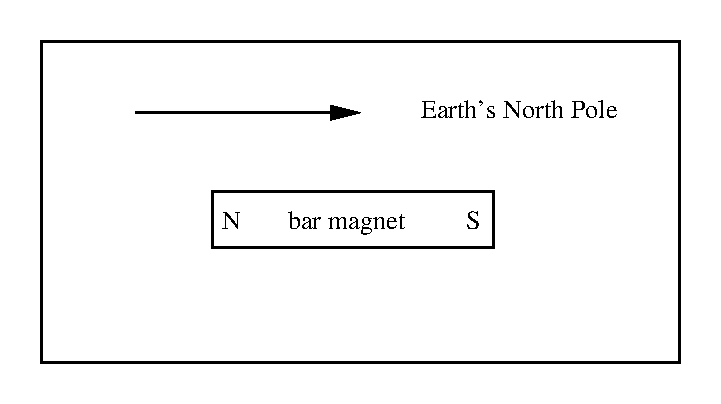
\includegraphics{magnetism_2_fig_1.eps}} \par}
%\vspace{0.3cm}

\begin{enumerate}
\item Connect the three capacitors in series with the sine wave generator.
\item Set the sine wave generator to 200 Hz (not critical) and adjust the
amplitude so that the output measures 5 to 6 volts as measured with the
digital multimeter set for \underline{AC volts}.
\item Using the multimeter, measure $V$ for the sine wave generator and also
for each of the individual capacitors (all with uncertainties) and
list them here. Don't forget units.\vspace{20mm}

\item Calculate the total voltage and its uncertainty from the first equation
above and compare with your measured value.  Do they agree?\vspace{30mm}

\item Assuming 10 percent uncertainties on each of the capacitances,
calculate the equivalent capacitance and its uncertainty from the second
equation above. (Note: To calculate the uncertainty we assume that if the value
 of each capacitor is known to 10 percent, then the value of 1/C for 
that capacitor is also known to 10 percent.) \vspace{45mm}

\item Calculate the total charge for the circuit (and its uncertainty) from
$Q = CV$.\vspace{30mm}

\item \textbf{Prediction:} How will the charge on the individual capacitors
compare with the total charge calculated above?\vspace{15mm}

\item Calculate the charge on each capacitor (and its uncertainty) and compare 
with the total. Do the results agree with your prediction?
\end{enumerate}
